%@author Brandon Roberts, Nate Olderman, Billy Rathje, DJ Maguddayao, Kyle Dybdal
%@date 9/23/13

\documentclass[12pt]{article}
\usepackage{graphicx}

\begin{document}

%-------------------------------------------------------------------------------------------------------------
% TITLE PAGE
%-------------------------------------------------------------------------------------------------------------

\begin{titlepage}
	\vspace*{\fill} %leave out given verticle space in a document
	\begin{center}
		{\Huge Story Creator Requirements Specification}\\ [0.5cm]	%make title huge and have .5cm space in between
		{\Large Brandon Roberts, Nate Olderman, Billy Rathje, DJ Maguddayao, Kyle Dybdal}\\[0.4cm]
		\today %put the date that the data is compiled
	\end{center}
	\vspace*{\fill}
\end{titlepage}

%-------------------------------------------------------------------------------------------------------------
%ABSTRACT/SUMMARY
%-------------------------------------------------------------------------------------------------------------
\section{Summary}
This SRS describes the requirements and specifications for the Story Creator module of the edith software, a system to help younger students learn to program. \\

======= \\ \\
%<<<<<<< HEAD
This SRS describes the requirements and specifications for the Story Creator module of the Edith software, a system to help younger students learn to program. The Story Creator module is used to combines the Sharing Framework, Object Creator, Visual Editor and Animation module in order to create a holistic view of Edith.  \\

======= \\ \\
This SRS describes the requirements and specifications for the Story Creator module of the Edith software, a system to help younger students learn to program.


%-------------------------------------------------------------------------------------------------------------
%INTRODUCTION
%-------------------------------------------------------------------------------------------------------------

\section{Introduction}%Create a section for the introduction
	\subsection{Edith}
	%adding this section to the beginning because he asks for description of the overall product in intro -Nate
	Edith will be a web-based, educational system designed to help younger students develop an interest in and learn about programming. The user will be able to create a "story" by dragging and dropping objects, giving the objects animations, and creating ways for the user or other users to interact with their story. By doing this, students will be able to learn how relationships among objects work in programming.
	\subsection{Scope}
	%%Tried to get rid of all the "fluff" -DJ
	The Story Creator module is intended to function as a display that integrates the work of the Animation System module and Visual Editor module in order to allow the user to create an animated story.  This module will employ the Visual Editor and Animation System module to interact with objects that are given by the Object Creator through a user interface combining the displays of the Animation System and Visual Editor module.  Story creator will add extra functionality to the Visual Editor and Animation System modules to interact with the Object Creator module in order to specify actions performed by the objects given by the Object Creator module.\
	\subsection{Purpose}
	%basically rewrote this section while trying to find the best way to describe the purpose of our team -Nate
	The purpose of the Story Creator section of the Edith software is to ensure that each other piece of the software can work together as a cohesive whole. This will be done through the user interface by providing a way for the user to select objects to choose actions and animations for each object. From there, the user will be able to interact in different ways with the animated objects that they have created and then finalize the "story" they have created so they can keep it or share it among friends. Story creator will construct these interactions between the pieces as well as a pleasant display view for the user.
	
%********	Next Team Member!  I ended here in the introduction.  I think it is almost/mainly done.  It will need some tweaks revision later on. ~Brandon ******************************
	
%-------------------------------------------------------------------------------------------------------------
%FUNCTIONAL REQUIREMENTS/USE CASES
%-------------------------------------------------------------------------------------------------------------
\section{Functional Requirements/Use Cases}
\subsection{"Navigate Story Files"}
\begin{itemize}
	\item Actor: The storyteller 
	\item Preconditions/Assumptions: No preconditions.
	\item Flow of Events: \\
	 	\ - User will open program. \\
		\ - 3.2 "Start a new story file" \\
		\ - 3.3 "Save the story" \\
		\ - 3.4 "Close the story"
	\item Alternatives: None
	\item Postconditions: None
\end{itemize}

	\subsection{"Start a new story file"}
\begin{itemize}
	\item Actor: The storyteller 
	\item Preconditions/Assumptions: No preconditions.
	\item Flow of Events: \\
		\ - User wants to create a new story. \\
		\ - User will select an option to create a new story.
	
	\item Alternatives: A previously created story may already be opened, in that case the user will close the story and proceed with the second event.
	\item Postconditions: The program will be ready for the user to create a story.
\end{itemize}

%%I'd assume that if nothing is there nothing is saved -DJ
		\subsection{"Save a story"}
\begin{itemize}
	\item Actor: The storyteller 
		\item Preconditions/Assumptions: A story has been created.
	\item Flow of Events: \\
	\	- User selects a "save story" option. \\
	\	- A representation of the story and its objects, scripts, and settings is sent to the Sharing Framework.
	\item Alternatives: If the story has never been saved before, the story editor will prompt
	the user to "save as."
	\item Postconditions: The story is saved to the local computer.
\end{itemize}
	
		\subsection{"Close a story"}
\begin{itemize}
	\item Actor: The storyteller
		\item Preconditions/Assumptions: A story is open at the time.
	\item Flow of Events: \\
	\	- The user selects an option to close the story. \\
	\	- The story is removed from the story editor. \\
	\	- Animations, scripts, and objects associated with the story are cleared from their respective editors.
	\item Alternatives: If the story is not saved, the story editor will prompt the user to
	save the story. If new objects, animations, or scripts have been created specifically for this
	story and have not been saved, the story editor will also prompt the user to save these
	new components.
	\item Postconditions: None.
\end{itemize}
	
	\subsection{"Create an object"}
\begin{itemize}
	\item Actor: The storyteller
	% changed from program is open to scene is open -BR
	\item Preconditions/Assumptions: A scene is open. 
	\item Flow of Events: \\
	 	\ - Storyteller wants to create an object in their story. \\
	 	\ - Storyteller will go to the Object Creator screen. \\
		\ - Storyteller will select an option to create an object. \\
		\ - Storyteller will use the mouse to drag the object. \\
		\ - Storyteller will choose where to place the object. \\
		\ - Storyteller will drop the object in that place.
	\item Alternatives: Object may not be compatible with some other objects/animations already in story, in that case user will choose whether to delete the old object or not create the new one.
	\item Postconditions: The program will display one additional object than it did before.
\end{itemize}

%********	Next Team Member!  This is where I ended, I went for simple so there  would be other possibilities for use cases. If it ends up with more possibilities than we thought of when we were together as a group this can be consolidated and made to be more complex use cases -Nate ******************************

	\subsection{"Remove an object"}
\begin{itemize}
	\item Actor: The storyteller
	\item Preconditions/Assumptions: At least one object is in the scene.
	\item Flow of Events: \\
	\	- User selects an option to delete objects. \\
	\	- User selects the object to delete. \\
	\	- The object disappears  from the scene.
	\item Alternatives: None.
	\item Postconditions: The program will display one fewer object than it did before.
\end{itemize}

	\subsection{"Move an object"}
\begin{itemize}
	\item Actor: The storyteller
		\item Preconditions/Assumptions: At least one object is in the scene.
	\item Flow of Events: \\
	\	- User selects an option to move objects. \\
	\	- User drags the object from its original location to a new one. (This is not an animation)
	\item Alternatives: If the user attempts to drag the object outside of the scene, the object
	will stay within the scene frame's boundaries.
	\item Postconditions: None.
\end{itemize}

	%--- I'm not sure if these should be longer... Right now there's not much 
	% I can think of for event flow besides interacting with the visual editor.
	
	\subsection{"Develop or edit a script"}
\begin{itemize}
		\item Actor: The storyteller
		\item Preconditions/Assumptions: None.
	\item Flow of Events: \\
	\	- Storyteller interacts with the visual editor to develop a new script. \\
	\   - Storyteller selects a specific action which is an individual script (All of the scripts interact a main loop) \\
	
	\item Alternatives: 3.9 "Delete a script"
	\item Postconditions: A script is added to the visual editor's list of scripts.
\end{itemize}

	\subsection{"Delete a script"}
\begin{itemize}
		\item Actor: The storyteller
		\item Preconditions/Assumptions: There is a script active.
	\item Flow of Events: \\
	\	- User interacts with the visual editor to delete a script.
	\item Alternatives: None.
	\item Postconditions: A script in the visual editor's list of scripts is removed.
\end{itemize}
	%------
	
	% Another question. If the user makes objects or scripts, can they reuse them in 
	% other scenes, or just in the present scene? I'm leaving both options open here,
	% and generalizing to just say that the object or script is "saved." -???
	%I'd assume that an object made can be reused.  No clue.  Someone else confirm?  -DJ
	\subsection{"Save an object or script"}
\begin{itemize}
	\item Actor: The storyteller
		\item Preconditions/Assumptions: The user has created a new object or script.
	\item Flow of Events: \\
	\	- The user wants to save an object or script for reuse. \\
	\	- A representation of the object or script is saved.
	\item Alternatives: If the story has never been saved before, the story editor will prompt
	the user to "save as."
	\item Postconditions: The object or script is available for reuse in the scene. It can
	also be made available for reuse in other scenes.
\end{itemize}
	
	\subsection{"Animate an object"}
\begin{itemize}
	\item Actor: The storyteller
		\item Preconditions/Assumptions: At least one object is in the scene and one script is in the visual editor.
	\item Flow of Events: \\
	\	- User selects a script from the visual editor. \\
	\	- User drags or otherwise attaches the script to an object in the scene.
	\item Alternatives: None.
	\item Postconditions: The object has an associated script/animation.
\end{itemize}


	\subsection{"Play story"}
\begin{itemize}
	\item Actor: The storyteller
		\item Preconditions/Assumptions: A 'story' is present.
	\item Flow of Events: \\
	\	- Storyteller selects a "play scene" option. \\
	\	- The story plays for the storyteller in the animation viewer at the beginning.
	\item Alternatives: The storyteller may interrupt playback with a variety
	of options, including stop, fast-forward, or rewind. The playback system will respond
	to these options. In the case of "stop," the scene playback will cancel. In the case of
	fast-forward or rewind, the scene will progress forward or backward more rapidly as long
	as the storyteller continues to select the fast-forward or rewind option.
	\item Postconditions: None.	
\end{itemize}

		\subsection{"Share a story"}
\begin{itemize}
	\item Actor: The storyteller
		\item Preconditions/Assumptions: There is a story present.
	\item Flow of Events: \\
	\	- User selects a "publish story option." \\
	\	- The story is converted to a representation that the sharing framework can read. \\
	\	- The story representation is sent to the sharing framework so that it can share the scene.
	\item Alternatives: If the story is not saved, or changes have been made since the last save,
	the story editor will prompt the user to save the story before sharing it.
	\item Postconditions: None.
\end{itemize}

%-------------------------------------------------------------------------------------------------------------
%NON-FUNCTIONAL REQUIREMENTS
%-------------------------------------------------------------------------------------------------------------
\section{Nonfunctional Requirements}
	\subsection{"Ease of Use"}
	The system should be easy for novices to use. One test of the system's usability is the
	number of errors made per hour of use. An "error" is defined as the user selecting the
	wrong options for: \\ \\
		\indent a) adding, editing, or deleting an object \\
		\indent b) attaching a script/animation to an object \\
		\indent c) saving and sharing the story \\
		\indent d) playing back the story. \\ \\
	The number of errors made by experienced users may differ significantly from those made
	by first-time or novice user. An experienced user should make no more than 3-5 errors per 			hour. While there is some complexity to the story editor, an experienced user should not
	have trouble knowing which options to choose to add objects or play the scene, for example.
	In comparison to the rest of the system, the story editor should be relatively similar to
	navigate, like a programming IDE or video editing system. Novice users may make many
	more errors when initially learning the system, but the system should not be frustrating to
	learn because it is designed to engage novice programmers and to make the task of programming
	feel simple and intuitive. Anything beyond 5-15 errors within 1-3 hours of use would be too 			many.
	
%============ To the next team member! I added in several new use cases...
% it may be that we can consolidate several cases into one, for example,
% all of the object cases - add object/edit object/delete object could
% maybe be combined into one case. I also added a nonfunctional requirement.
% I think they're almost done, but will need some edits and revisions
% I'll make another pass later. -Billy
%===========

%-------------------------------------------------------------------------------------------------------------
%GLOSSARY/REFERENCES
%-------------------------------------------------------------------------------------------------------------
\section{Glossary}
\begin{itemize}
\item Script:  A small program made in the visual editor that controls the object or scene event to be displayed.


\begin{figure}[ht!]
\centering
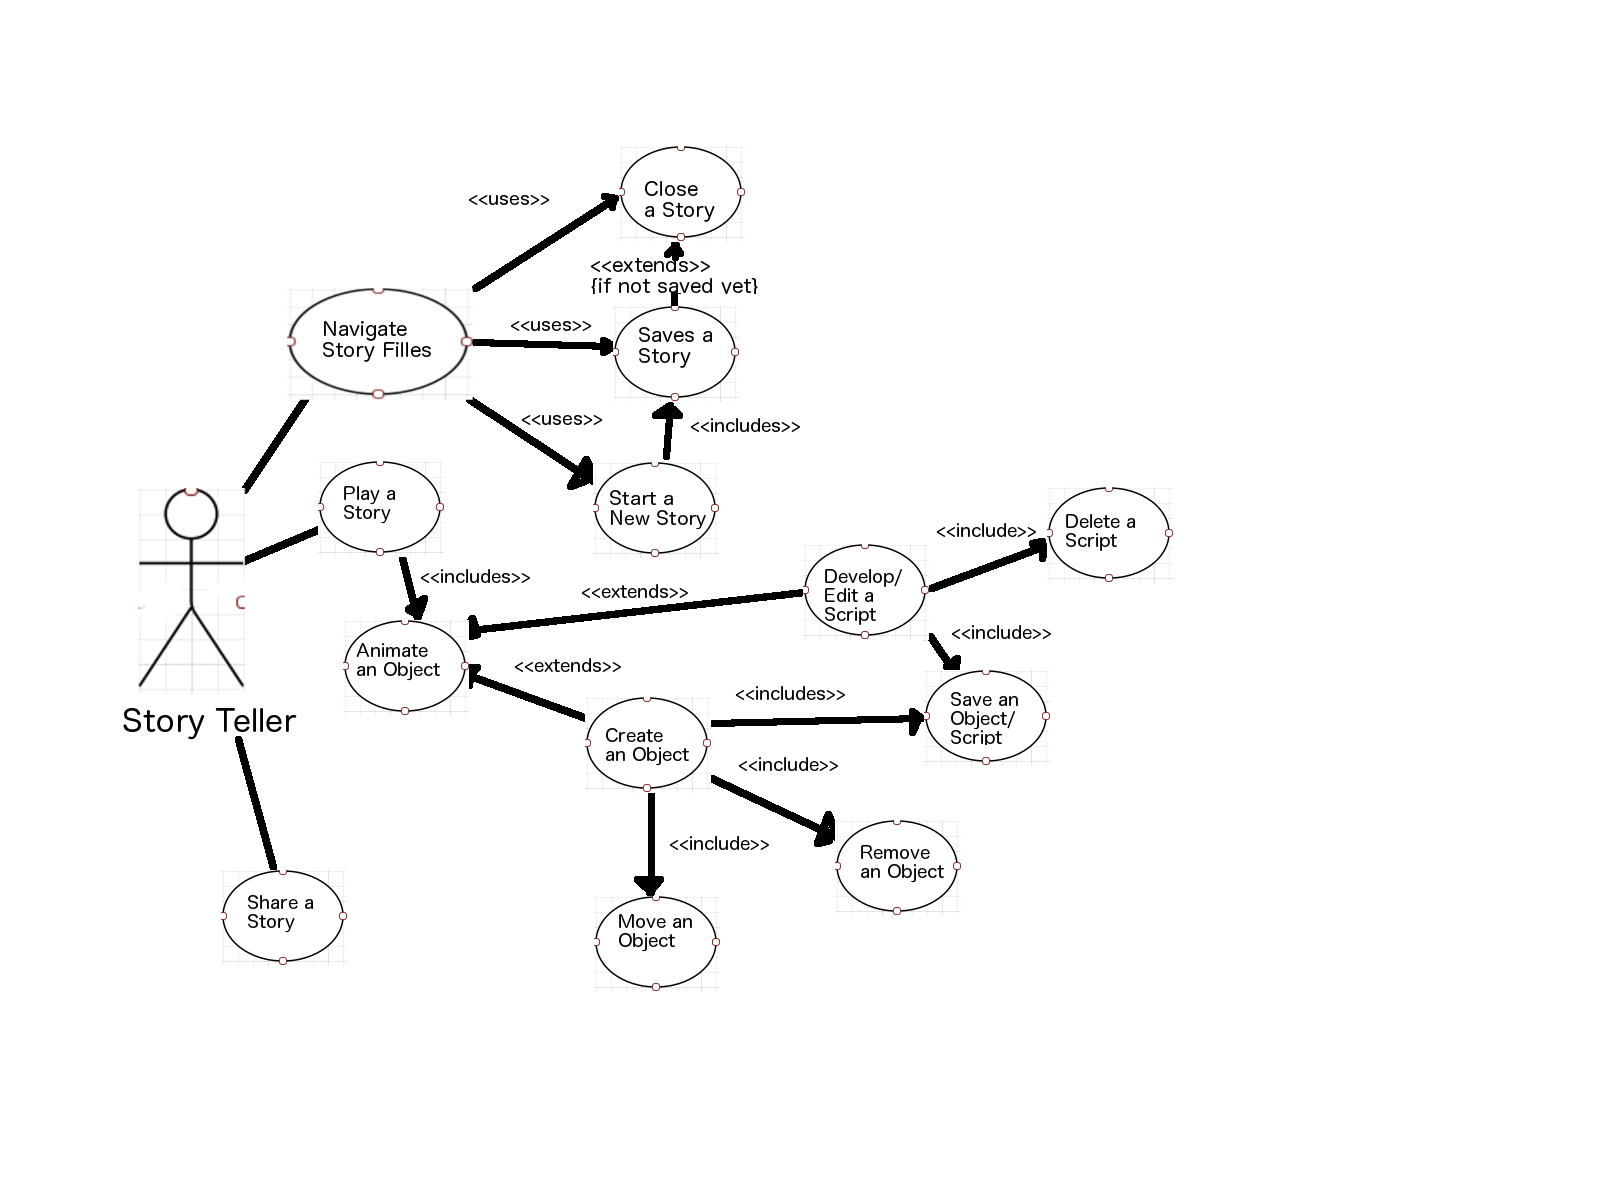
\includegraphics[width=200mm]{Story Creator FlowChart.png}
\caption{Use Case Diagram}
\label{overflow}
\end{figure}






\end{itemize}

\end{document}